\section{Chomp!}
	\sectionstart{The third game}{Math has never been this exciting (or delicious) \emoji{Images/ChocolateBarEmoji}}
	\begin{namedframe}{What's the game?}
		Chomp is played on a rectangular grid, such as squares of a candy bar.
		The lower left square is considered \alert{poison}.
		Players take turns picking a square.
		With each choice, all squares above and to the right of the picked square are no longer available -- they are eaten.
		The person forced to take the \alert{poison} square loses.
		\begin{center}
			\includegraphics[width=0.6\textwidth]{Images/Chomp1}
		\end{center}
	\end{namedframe}
	\begin{namedframe}{Let's play! ($4 \times 6$ board)}
		\begin{center}
			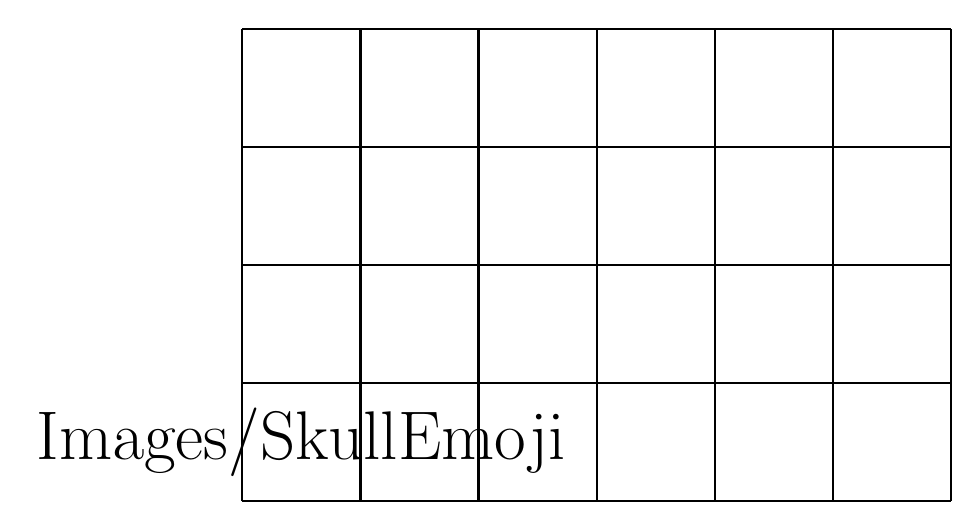
\begin{tikzpicture}
				\draw[step=1.5cm,black,thick] (0,0) grid(6 * 1.5,4 * 1.5);
				\draw (0.75,0.75) node {\Huge\emoji{Images/SkullEmoji}};
			\end{tikzpicture}
		\end{center}
	\end{namedframe}
	\begin{namedframe}{Is there a winning strategy? (Or, why this game so cool.)}
		Yes!
		\begin{itemize}[<+(1)->]
			\item The first player has a winning strategy for any finite grid.
				\begin{itemize}
					\item They can take any move that the second can player can make, that would result in winning.
					\begin{itemize}
						\item We can think of this as strategy stealing!
					\end{itemize}
				\end{itemize}
		\end{itemize}
		\pause
		The real question is\ldots
	\end{namedframe}
	\begin{namedframe}{What is the winning strategy?}
		\begin{itemize}[<+->]
			\item Does anyone know one right away?
			\item No!
			\item Let's analyze some cases!
		\end{itemize}
	\end{namedframe}
	\begin{namedframe}{$n \times n$ grid}
		\begin{itemize}[<+->]
			\item What's the strategy here?
			\item Make an ``L'', and then take symmetrical moves!
		\end{itemize}
		\begin{center}
			\includegraphics[width=0.5\textwidth]{Images/Chomp2}
		\end{center}
	\end{namedframe}
	\begin{namedframe}{$2 \times n$ grid}
		\begin{itemize}[<+->]
			\item What's the strategy here?
			\item Make sure that player 2 encounters a rectangle\ldots{} with a square missing!
		\end{itemize}
		\begin{center}
			\includegraphics[width=\textwidth]{Images/Chomp3}
		\end{center}
	\end{namedframe}
	\begin{namedframe}{What is the winning strategy?}
		\begin{itemize}[<+(1)->]
			\item Just because there is always a winning strategy for player 1 doesn't mean that we know what it is!
			\item We know the strategy for $n \times n$ and $2 \times n$, as well as particular small grids\ldots{} but not all\ldots
			\begin{itemize}
				\item In 2002, Steven Byrnes (a high school senior!!) solved the $3 \times n$ case and won over $\$100\,000$
				\item Computers can calculate winning moves for grids of reasonable size
			\end{itemize}
		\end{itemize}
	\end{namedframe}
	\begin{namedframe}{Some cool extensions}
		\begin{columns}
			\begin{column}{0.5\textwidth}
				\begin{itemize}
					\item $3$D or $n$D chomp
					\item Infinite/ordinal chomp:
					\begin{itemize}
						\item Here is how player ``Too'' can win on a $2 \times \omega$ board
					\end{itemize}
				\end{itemize}
			\end{column}
			\begin{column}{0.5\textwidth}
				\includegraphics[width=\textwidth]{Images/Chomp3D}
			\end{column}
		\end{columns}
		\begin{center}
			\includegraphics[width=0.75\textwidth]{Images/Chomp4}
		\end{center}
	\end{namedframe}
